% Figure 2 v2 — ABM Forward Simulation Pipeline
% Focus: agent dispatch + BPR closure method details (matching Figure 1's
% encoder-level granularity).
%
% Layout:
%   Top ribbon:    Setup (receive frozen Θ + do(X) intervention)
%   Stage B:       Agent dispatch — 6 fine-grained sub-modules
%   Stage C:       BPR + MSA closure — 7 fine-grained sub-modules
%   Bottom ribbon: Outputs (welfare assessment)
%
% Compile:  pdflatex figure2_abm_v2.tex

\documentclass[border=8pt]{standalone}

\usepackage[T1]{fontenc}
\usepackage{lmodern}
\usepackage{amsmath, amssymb}
\usepackage{tikz}
\usepackage{xcolor}
\usepackage{graphicx}

\usetikzlibrary{
  positioning, arrows.meta, shapes.geometric, calc, fit, backgrounds,
  matrix, decorations.pathmorphing,
}

% ── Stage colour palette ────────────────────────────────────────────────
\definecolor{ribbonBg}    {HTML}{F1F5F9}
\definecolor{ribbonBanner}{HTML}{475569}
\definecolor{stageBBg}    {HTML}{FCE4C7}    % light orange — agent dispatch
\definecolor{stageBBanner}{HTML}{C2410C}
\definecolor{stageCBg}    {HTML}{F5E6D8}    % light brown — BPR + MSA
\definecolor{stageCBanner}{HTML}{92400E}
\definecolor{outputBg}    {HTML}{D6EBE8}
\definecolor{outputBanner}{HTML}{0F766E}

\definecolor{cFlow}       {HTML}{E07A5F}
\definecolor{cBPR}        {HTML}{F59E0B}
\definecolor{cText}       {HTML}{1F2937}
\definecolor{cMuted}      {HTML}{6B7280}
\definecolor{cBorder}     {HTML}{CBD5E1}
\definecolor{cIO}         {HTML}{0F766E}

\definecolor{cParEnc}   {HTML}{475569}
\definecolor{cParBeta}  {HTML}{C44E52}
\definecolor{cParGamma} {HTML}{F59E0B}
\definecolor{cParDelta} {HTML}{0E7490}
\definecolor{cParKappa} {HTML}{8172B2}

\definecolor{cAgentWalk}   {HTML}{10B981}
\definecolor{cAgentTransit}{HTML}{F59E0B}
\definecolor{cAgentCar}    {HTML}{3B82F6}

\begin{document}

\begin{tikzpicture}[
  font=\sffamily\small,
  thick,
  >={Stealth[length=4pt, width=4pt]},
  every node/.style={align=center, text=cText},
  %
  rowframe/.style={
    draw=none, fill=#1, rounded corners=6pt,
    inner xsep=8pt, inner ysep=10pt,
  },
  rowbanner/.style={
    fill=#1, text=white, font=\sffamily\bfseries\small,
    rounded corners=4pt, inner sep=6pt,
  },
  modB/.style={
    draw=stageBBanner, fill=white, line width=0.7pt,
    rounded corners=3pt, inner sep=5pt,
    font=\sffamily\footnotesize,
  },
  modC/.style={
    draw=stageCBanner, fill=white, line width=0.7pt,
    rounded corners=3pt, inner sep=5pt,
    font=\sffamily\footnotesize,
  },
  arrFwd/.style={->, line width=1.4pt, draw=cFlow},
  arrInner/.style={->, line width=0.8pt, draw=cText!70},
  arrBPR/.style={->, line width=1.0pt, draw=cBPR, dashed},
  arrlbl/.style={font=\sffamily\scriptsize\itshape, text=cMuted, fill=white,
                 inner sep=1pt, midway},
]

% ════════════════════════════════════════════════════════════════════════
%  TOP RIBBON · SETUP (frozen Θ + counterfactual intervention)
% ════════════════════════════════════════════════════════════════════════

\begin{scope}[local bounding box=ribbontop]
  % 5 frozen-param mini-pills (linked from Figure 1)
  \node[draw=cParEnc, fill=cParEnc!15, rounded corners=2pt, line width=0.5pt,
         minimum width=24mm, minimum height=8mm,
         font=\sffamily\tiny, text=cParEnc, align=center,
         anchor=north west] (penc) at (0, 0) {Encoder weights\\\tiny 33{,}026};
  \node[draw=cParBeta, fill=cParBeta!15, rounded corners=2pt, line width=0.5pt,
         minimum width=24mm, minimum height=8mm,
         font=\sffamily\tiny, text=cParBeta, align=center,
         anchor=north west] (pbeta) at (26mm, 0) {Time sensitivity\\\tiny 72};
  \node[draw=cParGamma, fill=cParGamma!15, rounded corners=2pt, line width=0.5pt,
         minimum width=24mm, minimum height=8mm,
         font=\sffamily\tiny, text=cParGamma, align=center,
         anchor=north west] (pgamma) at (52mm, 0) {Distance decay\\\tiny 1};
  \node[draw=cParDelta, fill=cParDelta!15, rounded corners=2pt, line width=0.5pt,
         minimum width=24mm, minimum height=8mm,
         font=\sffamily\tiny, text=cParDelta, align=center,
         anchor=north west] (pdelta) at (78mm, 0) {Occ.\ matching\\\tiny 2};
  \node[draw=cParKappa, fill=cParKappa!15, rounded corners=2pt, line width=0.5pt,
         minimum width=24mm, minimum height=8mm,
         font=\sffamily\tiny, text=cParKappa, align=center,
         anchor=north west] (pkappa) at (104mm, 0) {Tier scaling\\\tiny 2};

  % do(X) interventions
  \node[draw=ribbonBanner, fill=yellow!10, rounded corners=2pt, line width=0.6pt,
         minimum width=58mm, minimum height=8mm,
         font=\sffamily\tiny, text=cText, align=center,
         anchor=north west] (doxa) at (140mm, 0)
        {do$(X^{\text{static}})$ — Sc.\,A: OOC $+$65k jobs};
  \node[draw=ribbonBanner, fill=yellow!10, rounded corners=2pt, line width=0.6pt,
         minimum width=68mm, minimum height=8mm,
         font=\sffamily\tiny, text=cText, align=center,
         anchor=north west] (doxb) at (200mm, 0)
        {do$(X^{\text{dyn}})$ — Sc.\,B: peak $\!\times\!0.5$, shoulder $\!\times\!1.5$};
\end{scope}

\begin{pgfonlayer}{background}
  \node[rowframe=ribbonBg, fit=(ribbontop)] (frameTop) {};
\end{pgfonlayer}
\node[rowbanner=ribbonBanner, anchor=north west]
  at ($(frameTop.north west)+(8pt, 0pt)$)
  {\textsc{Setup}\;\,\textmd{\itshape — frozen $\Theta\bigstar$ from Fig.~1 (no re-fit) $+$ counterfactual intervention $\mathrm{do}(X)$ on the input tensor}};

% ════════════════════════════════════════════════════════════════════════
%  STAGE B · AGENT DISPATCH (6 sub-modules)
% ════════════════════════════════════════════════════════════════════════

\begin{scope}[local bounding box=stageB, shift={(0, -22mm)}]

  % ① Sample N agents
  \node[modB, anchor=north west] (agt) at (0, 0)
    {\begin{minipage}{50mm}
      \centering\textbf{\textcolor{stageBBanner}{\textcircled{\scriptsize 1} Sample $N$ agents}}\\[1pt]
      \scriptsize\textcolor{cIO}{IN: $\pi_m, \pi_k$, population}\;\;\textcolor{cIO}{OUT: $N$ tuples}\\[3pt]
      \begin{tikzpicture}[baseline=0]
        \foreach \i/\xoff/\col in
          {1/0/cAgentWalk, 2/4mm/cAgentTransit, 3/8mm/cAgentCar,
           4/12mm/cAgentWalk, 5/16mm/cAgentTransit, 6/20mm/cAgentCar,
           7/24mm/cAgentTransit, 8/28mm/cAgentCar, 9/32mm/cAgentWalk}{
          \node[circle, fill=\col, minimum size=1.4mm, inner sep=0pt]
                at (\xoff, 0) {};
        }
        \node[font=\sffamily\tiny, text=cText, anchor=west] at (-2mm, -4mm)
              {tuple $(i_n, t_n, m_n, k_n)$};
        \node[font=\sffamily\tiny, text=cMuted, anchor=west] at (-2mm, -7mm)
              {drawn from $\pi_m(i)\!\times\!\pi_k(i)$};
      \end{tikzpicture}
    \end{minipage}};

  % ② Fetch personal parameters
  \node[modB, anchor=north west] (fetch) at (54mm, 0)
    {\begin{minipage}{56mm}
      \centering\textbf{\textcolor{stageBBanner}{\textcircled{\scriptsize 2} Fetch personal parameters}}\\[1pt]
      \scriptsize\textcolor{cIO}{IN: $(m_n, k_n)$, frozen $\Theta$}\;\;\textcolor{cIO}{OUT: $(\beta, \kappa, \delta)$ for agent $n$}\\[3pt]
      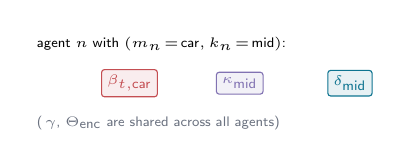
\begin{tikzpicture}[baseline=0]
        \node[font=\sffamily\tiny, anchor=west] at (-1mm, 0)
              {agent $n$ with $(m_n\!=\!\text{car}, k_n\!=\!\text{mid})$:};
        \node[draw=cParBeta, fill=cParBeta!10, rounded corners=1pt, line width=0.4pt,
               font=\sffamily\tiny, text=cParBeta, inner sep=2pt]
             at (12mm, -5mm) {$\beta_{t,\text{car}}$};
        \node[draw=cParKappa, fill=cParKappa!10, rounded corners=1pt, line width=0.4pt,
               font=\sffamily\tiny, text=cParKappa, inner sep=2pt]
             at (26mm, -5mm) {$\kappa_{\text{mid}}$};
        \node[draw=cParDelta, fill=cParDelta!10, rounded corners=1pt, line width=0.4pt,
               font=\sffamily\tiny, text=cParDelta, inner sep=2pt]
             at (40mm, -5mm) {$\delta_{\text{mid}}$};
        \node[font=\sffamily\tiny, text=cMuted, anchor=west] at (-1mm, -10mm)
              {(\,$\gamma$, $\Theta_{\text{enc}}$ are shared across all agents)};
      \end{tikzpicture}
    \end{minipage}};

  % ③ Compute utility U_n
  \node[modB, anchor=north west] (util) at (114mm, 0)
    {\begin{minipage}{82mm}
      \centering\textbf{\textcolor{stageBBanner}{\textcircled{\scriptsize 3} Compute utility $U_{n,j}$}}\\[1pt]
      \scriptsize\textcolor{cIO}{IN: $V'_{j,t}$, agent params}\;\;\textcolor{cIO}{OUT: $U_{n,j}$ for each $j$}\\[3pt]
      \scriptsize $U_{n,j}\!=\!\alpha V'_{j,t} + \beta_{t,m_n}\kappa_{k_n} t_{ij}^{(m_n)} + \gamma\log d + \delta_{k_n}\mathrm{OccM}$\\[2pt]
      \tiny\textcolor{cMuted}{shared encoder pass: $V'_{j,t}\!=\!\text{enc}(X^{\text{perturbed}}; \Theta_{\text{enc}}^{\,\bigstar})$}
    \end{minipage}};

  % ④ Add Gumbel ε
  \node[modB, anchor=north west] (gumbel) at (200mm, 0)
    {\begin{minipage}{50mm}
      \centering\textbf{\textcolor{stageBBanner}{\textcircled{\scriptsize 4} Add Gumbel noise}}\\[1pt]
      \scriptsize\textcolor{cIO}{IN: $U_{n,j}$}\;\;\textcolor{cIO}{OUT: $U_{n,j} + \varepsilon_{n,j}$}\\[3pt]
      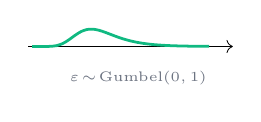
\begin{tikzpicture}[baseline=0]
        \draw[->, line width=0.3pt] (-2mm, 0) -- (24mm, 0);
        \draw[cAgentWalk, line width=1.0pt, smooth, samples=30, domain=-3:6]
              plot (\x*2.5mm + 6mm, {6mm * exp(-\x - exp(-\x))});
        \node[font=\sffamily\tiny, text=cMuted] at (12mm, -4mm) {$\varepsilon\!\sim\!\mathrm{Gumbel}(0,1)$};
      \end{tikzpicture}
    \end{minipage}};

  % ⑤ argmax → choice j*
  \node[modB, anchor=north west] (argmax) at (0, -36mm)
    {\begin{minipage}{82mm}
      \centering\textbf{\textcolor{stageBBanner}{\textcircled{\scriptsize 5} $j_n^* = \arg\max_j (U_{n,j} + \varepsilon_{n,j})$}}\\[1pt]
      \scriptsize agent picks ONE destination among $N\!=\!1725$ candidates\\[3pt]
      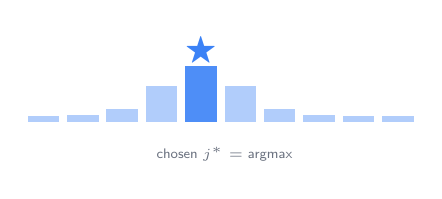
\begin{tikzpicture}[baseline=0]
        \foreach \k in {0,1,2,3,4,5,6,7,8,9}{
          \pgfmathsetmacro{\h}{0.6 + 4.5*exp(-0.5*(\k-4)*(\k-4))}
          \pgfmathtruncatemacro{\chosen}{ifthenelse(\k==4, 1, 0)}
          \fill[cAgentCar, opacity={0.4 + 0.5*\chosen}]
                (\k*5mm, 0) rectangle (\k*5mm + 4mm, \h*1.4mm);
        }
        \node[font=\sffamily\large, text=cAgentCar] at (4*5mm + 2mm, 9mm) {$\bigstar$};
        \node[font=\sffamily\tiny, text=cMuted] at (25mm, -4mm) {chosen $j^* = $ argmax};
      \end{tikzpicture}
    \end{minipage}};

  % ⑥ Aggregate F̂_ij,t
  \node[modB, anchor=north west] (aggr) at (88mm, -36mm)
    {\begin{minipage}{160mm}
      \centering\textbf{\textcolor{stageBBanner}{\textcircled{\scriptsize 6} Aggregate to $\widehat{F}_{ij,t}$}}\;\;\scriptsize\textcolor{cIO}{IN: $j_n^*$ for $n\!=\!1{:}N$}\;\;\textcolor{cIO}{OUT: hourly OD flow $\widehat{F}_{ij,t}$}\\[3pt]
      \scriptsize $\widehat{F}_{ij,t}=\sum_{n=1}^{N}\!\mathbb{1}[i_n\!=\!i,\,t_n\!=\!t,\,j_n^*\!=\!j]$\;\;
      \tiny\textcolor{cMuted}{number of agents with origin $i$, hour $t$ who chose destination $j$}
    \end{minipage}};

  % inner arrows
  \draw[arrInner] (agt.east) -- (fetch.west);
  \draw[arrInner] (fetch.east) -- (util.west);
  \draw[arrInner] (util.east) -- (gumbel.west);
  \draw[arrInner] (gumbel.south) |- ($(argmax.north)+(20mm, 0)$);
  \draw[arrInner] (argmax.east) -- (aggr.west);

\end{scope}

\begin{pgfonlayer}{background}
  \node[rowframe=stageBBg, fit=(stageB)] (frameStageB) {};
\end{pgfonlayer}
\node[rowbanner=stageBBanner, anchor=north west]
  at ($(frameStageB.north west)+(8pt, 0pt)$)
  {\textsc{Stage B · Agent dispatch}\;\,\textmd{\itshape — instantiate $N$ heterogeneous agents and run their per-agent destination choice}};

% ════════════════════════════════════════════════════════════════════════
%  STAGE C · BPR + MSA CLOSURE (7 sub-modules — congestion estimation)
% ════════════════════════════════════════════════════════════════════════

\begin{scope}[local bounding box=stageC, shift={(0, -120mm)}]

  % ⑦ Inflow aggregation
  \node[modC, anchor=north west] (inflow) at (0, 0)
    {\begin{minipage}{52mm}
      \centering\textbf{\textcolor{stageCBanner}{\textcircled{\scriptsize 7} Destination inflow}}\\[1pt]
      \scriptsize\textcolor{cIO}{IN: $\widehat{F}_{ij,t}$}\;\;\textcolor{cIO}{OUT: $\mathrm{Inflow}_{j,t}$}\\[3pt]
      \scriptsize $\mathrm{Inflow}_{j,t}\!=\!\sum_i \widehat{F}_{ij,t}$\\[2pt]
      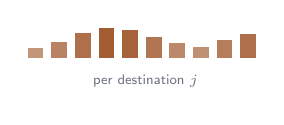
\begin{tikzpicture}[baseline=0]
        % deterministic inflow heights — peaks in middle, smaller at edges
        \foreach \k/\h/\op in
          {0/1.2/55, 1/2.0/65, 2/3.1/75, 3/3.8/85, 4/3.5/82,
           5/2.6/72, 6/1.8/62, 7/1.4/58, 8/2.2/68, 9/3.0/75}{
          \fill[stageCBanner!\op] (\k*3mm, 0) rectangle (\k*3mm + 2mm, \h mm);
        }
        \node[font=\sffamily\tiny, text=cMuted] at (15mm, -3mm) {per destination $j$};
      \end{tikzpicture}
    \end{minipage}};

  % ⑧ V/C ratio
  \node[modC, anchor=north west] (vc) at (56mm, 0)
    {\begin{minipage}{52mm}
      \centering\textbf{\textcolor{stageCBanner}{\textcircled{\scriptsize 8} V/C ratio}}\\[1pt]
      \scriptsize\textcolor{cIO}{IN: $\mathrm{Inflow}_{j,t}, C_j$}\;\;\textcolor{cIO}{OUT: $V/C$}\\[3pt]
      \scriptsize $V/C_{j,t}\!=\!\mathrm{Inflow}_{j,t} \,/\, C_j$\\[2pt]
      \tiny\textcolor{cMuted}{$C_j$\,=\,baseline daily inflow}\\
      \tiny\textcolor{cMuted}{$\times$ capacity scale (proxy)}
    \end{minipage}};

  % ⑨ BPR multiplier
  \node[modC, anchor=north west] (mult) at (112mm, 0)
    {\begin{minipage}{52mm}
      \centering\textbf{\textcolor{stageCBanner}{\textcircled{\scriptsize 9} BPR multiplier}}\\[1pt]
      \scriptsize\textcolor{cIO}{IN: $V/C$}\;\;\textcolor{cIO}{OUT: $r_{j,t}\!\geq\!1$}\\[3pt]
      \scriptsize $r_{j,t}\!=\!1\!+\!0.15\!\cdot\!(V/C)^4$\\[2pt]
      \tiny\textcolor{cMuted}{Sheffi 1985\;·\;capped at $2.5$}\\[2pt]
      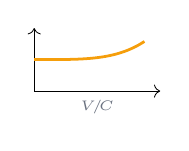
\begin{tikzpicture}[baseline=0]
        \draw[->, line width=0.3pt] (0, 0) -- (16mm, 0);
        \draw[->, line width=0.3pt] (0, 0) -- (0, 8mm);
        \draw[cBPR, line width=1.0pt, smooth, samples=20, domain=0:1.4]
              plot (\x*10mm, {(1 + 0.15*\x*\x*\x*\x)*4mm});
        \node[font=\sffamily\tiny, text=cMuted] at (8mm, -2mm) {$V\!/\!C$};
      \end{tikzpicture}
    \end{minipage}};

  % ⑩ Update t_car
  \node[modC, anchor=north west] (updt) at (168mm, 0)
    {\begin{minipage}{52mm}
      \centering\textbf{\textcolor{stageCBanner}{\textcircled{\scriptsize 10} Update $t_{ij}^{(\text{car})}$}}\\[1pt]
      \scriptsize\textcolor{cIO}{IN: $t_0^{(\text{car})}, r_{j,t}$}\;\;\textcolor{cIO}{OUT: $t^{(\text{car}),\text{cong}}$}\\[3pt]
      \scriptsize $t_{ij,t}^{(\text{car}),\text{cong}}\!=\!t_{ij,0}^{(\text{car})}\!\cdot\! r_{j,t}$\\[2pt]
      \tiny\textcolor{cMuted}{transit \& walk $t$ unchanged}
    \end{minipage}};

  % ⑪ MSA averaging
  \node[modC, anchor=north west] (msa) at (224mm, 0)
    {\begin{minipage}{56mm}
      \centering\textbf{\textcolor{stageCBanner}{\textcircled{\scriptsize 11} MSA averaging}}\\[1pt]
      \scriptsize\textcolor{cIO}{IN: $F^{(k)}, F^{\text{new}}$}\;\;\textcolor{cIO}{OUT: $F^{(k+1)}$}\\[3pt]
      \scriptsize $F^{(k+1)}\!=\!(1{-}\frac{1}{k})F^{(k)}\!+\!\frac{1}{k}\,F^{\text{new}}$\\[2pt]
      \tiny\textcolor{cMuted}{method of successive avgs}\\
      \tiny\textcolor{cMuted}{(Sheffi 1985 schedule)}
    \end{minipage}};

  % ⑫ Convergence check
  \node[modC, anchor=north west] (conv) at (0, -44mm)
    {\begin{minipage}{120mm}
      \centering\textbf{\textcolor{stageCBanner}{\textcircled{\scriptsize 12} Convergence check}}\\[1pt]
      \scriptsize relative gap = $\max_{ij}|t^{(k+1)}\!-\!t^{(k)}|\,/\,\overline{t^{(k)}}$\\[3pt]
      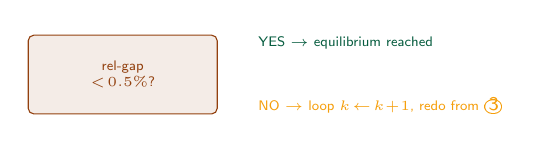
\begin{tikzpicture}[baseline=0]
        \node[draw=stageCBanner, rounded corners=2pt, fill=stageCBanner!10,
               minimum width=24mm, minimum height=10mm,
               font=\sffamily\tiny, text=stageCBanner, align=center] (rg) at (0, 0)
              {rel-gap\\$<\!0.5\%$?};
        \node[font=\sffamily\tiny, text=cAgentWalk!50!black, anchor=west] at (16mm, 4mm)
              {YES $\to$ equilibrium reached};
        \node[font=\sffamily\tiny, text=cBPR, anchor=west] at (16mm, -4mm)
              {NO $\to$ loop ${k\!\leftarrow\!k\!+\!1}$, redo from \textcircled{\scriptsize 3}};
      \end{tikzpicture}
    \end{minipage}};

  % ⑬ Equilibrium output
  \node[modC, anchor=north west] (eq) at (130mm, -44mm)
    {\begin{minipage}{150mm}
      \centering\textbf{\textcolor{stageCBanner}{\textcircled{\scriptsize 13} Equilibrium $\widehat{F}^{*},\,t^{(\text{car}),\text{eq}}$}}\\[1pt]
      \scriptsize converged flow + congested travel time\\[3pt]
      \scriptsize Sc.\,A: $\Delta\mathrm{inflow}\!=\!{+}414{\to}{+}261$ (37\% damping; converged in 30 iter)\\
      \scriptsize Sc.\,B: $t_{\text{car}}^{h08}{:}\,34.2{\to}32.7\,$min ($-4.4\%$; converged in 8 iter)
    \end{minipage}};

  % inner arrows
  \draw[arrInner] (inflow.east) -- (vc.west);
  \draw[arrInner] (vc.east) -- (mult.west);
  \draw[arrInner] (mult.east) -- (updt.west);
  \draw[arrInner] (updt.east) -- (msa.west);
  \draw[arrInner] (msa.south) |- ($(conv.north)+(56mm, 0)$);
  \draw[arrInner] (conv.east) -- (eq.west);

  % BPR feedback loop arrow back to Stage B (③ utility)
  \draw[arrBPR] ($(conv.north)+(40mm, 0)$) .. controls
                 ($(conv.north)+(40mm, 14mm)$) and
                 ($(conv.north)+(-40mm, 30mm)$) ..
                 node[arrlbl, near end, font=\sffamily\scriptsize\itshape, fill=white, text=cBPR]
                     {if NOT converged: re-run agent dispatch with new $t^{(\text{car})}$}
                 ($(conv.north)+(-40mm, 50mm)$);

\end{scope}

\begin{pgfonlayer}{background}
  \node[rowframe=stageCBg, fit=(stageC)] (frameStageC) {};
\end{pgfonlayer}
\node[rowbanner=stageCBanner, anchor=north west]
  at ($(frameStageC.north west)+(8pt, 0pt)$)
  {\textsc{Stage C · BPR $+$ MSA closure}\;\,\textmd{\itshape — destination-side congestion estimation, iterated to fixed-point equilibrium}};

% ════════════════════════════════════════════════════════════════════════
%  BOTTOM RIBBON · OUTPUTS
% ════════════════════════════════════════════════════════════════════════

\begin{scope}[local bounding box=ribbonout, shift={(0, -212mm)}]
  \node[draw=outputBanner, fill=white, rounded corners=2pt, line width=0.6pt,
         minimum width=84mm, minimum height=18mm,
         font=\sffamily\footnotesize, text=cText, align=center,
         anchor=north west] (a_i) at (0, 0)
        {\textbf{\textcolor{outputBanner}{Hansen accessibility}}\\\scriptsize $A_i\!=\!\sum_j E_j\,e^{\beta_{\text{car}} t_{ij}^{(\text{car}),\text{eq}}}$\\\tiny CBD-concentrated · max\,/\,p10 $\approx$\,25$\times$};
  \node[draw=outputBanner, fill=white, rounded corners=2pt, line width=0.6pt,
         minimum width=84mm, minimum height=18mm,
         font=\sffamily\footnotesize, text=cText, align=center,
         anchor=north west] (welfare) at (90mm, 0)
        {\textbf{\textcolor{outputBanner}{Welfare $\Delta$ Gini, Palma}}\\\scriptsize Sc.\,A regressive ($\Delta$Gini${+}1.3\%$)\\\scriptsize Sc.\,B progressive ($\Delta$Gini${<}0$)};
  \node[draw=outputBanner, fill=white, rounded corners=2pt, line width=0.6pt,
         minimum width=104mm, minimum height=18mm,
         font=\sffamily\footnotesize, text=cText, align=center,
         anchor=north west] (insight) at (180mm, 0)
        {\textbf{\textcolor{outputBanner}{Central policy finding}}\\\scriptsize same trained $\Theta$, opposite distributional verdicts\\\scriptsize $\Rightarrow$ temporal demand-shift dominates spatial supply-shift on welfare};
\end{scope}

\begin{pgfonlayer}{background}
  \node[rowframe=outputBg, fit=(ribbonout)] (frameOut) {};
\end{pgfonlayer}
\node[rowbanner=outputBanner, anchor=north west]
  at ($(frameOut.north west)+(8pt, 0pt)$)
  {\textsc{Outputs · counterfactual welfare assessment}};

% ════════════════════════════════════════════════════════════════════════
%  MAIN VERTICAL FLOW ARROWS
% ════════════════════════════════════════════════════════════════════════

\draw[arrFwd] ($(frameTop.south)+(0, 0)$) --
              node[arrlbl, fill=white, font=\sffamily\small\bfseries]
                  {$X^{\,\prime}+\Theta\!\bigstar$ frozen}
              ($(frameStageB.north)+(0, 0)$);
\draw[arrFwd] ($(frameStageB.south)+(0, 0)$) --
              node[arrlbl, fill=white, font=\sffamily\small\bfseries]{$\widehat{F}_{ij,t}$}
              ($(frameStageC.north)+(0, 0)$);
\draw[arrFwd] ($(frameStageC.south)+(0, 0)$) --
              node[arrlbl, fill=white, font=\sffamily\small\bfseries]{$\widehat{F}^{*}, t_{\text{eq}}$}
              ($(frameOut.north)+(0, 0)$);

% ════════════════════════════════════════════════════════════════════════
%  Title and footer
% ════════════════════════════════════════════════════════════════════════

\node[font=\sffamily\bfseries\Large, anchor=south west, text=cText]
  at ($(frameTop.north west)+(0, 8mm)$)
  {Figure 2 — ABM Forward Simulation Pipeline};
\node[font=\sffamily\itshape\large, anchor=south west, text=cMuted]
  at ($(frameTop.north west)+(0, 4mm)$)
  {agent-based deployment with destination-side BPR congestion closure};

\node[font=\sffamily\scriptsize\itshape, text=cMuted, anchor=north west,
       text width=300mm]
  at ($(frameOut.south west)+(0, -6pt)$)
  {Stage~B instantiates $N$ heterogeneous agents, each fetching their personal $(\beta_{t,m_n}, \kappa_{k_n}, \delta_{k_n})$ from frozen $\Theta$ and choosing one destination via Gumbel-max.\;
   Stage~C then closes the destination-side congestion loop (BPR multiplier on car) iteratively via MSA until rel-gap $<\!0.5\%$.\;
   The same trained $\Theta$ from Figure~1 is used; Stage~C does \emph{no} re-fitting.};

\end{tikzpicture}

\end{document}
